\documentclass{article}


\title{Revision: simulation study}



\usepackage[style=numeric,giveninits=true,maxbibnames=99,url=false,doi=false,isbn=false]{biblatex}
\usepackage{mathrsfs}
\usepackage{biblatex}
\usepackage{algorithm}
\usepackage{algorithmic}
\usepackage{amsthm}
\usepackage{amsmath}
\usepackage{bm}
\usepackage{comment}
\usepackage{xcolor}
\usepackage{amssymb}
\usepackage{hyperref}
\hypersetup{colorlinks,linkcolor=blue,anchorcolor=blue,citecolor=blue}
\usepackage{geometry}
\usepackage{appendix}
\usepackage{graphicx}
\usepackage{multicol}
\usepackage{hyperref}
\usepackage{booktabs}
\usepackage{multirow}
\usepackage{threeparttable}
\usepackage{caption}
\usepackage{bbm}
\usepackage{subcaption}
\newcommand{\vssmall}{\vspace{1mm}}


% (1) choose a font that is available as T1
% for example:
\usepackage{lmodern}

% (2) specify encoding
\usepackage[T1]{fontenc}

% (3) load symbol definitions
\usepackage{textcomp}


\geometry{a4paper,scale=0.7}
\addbibresource{ref.bib} 






\def\AIC{\textsc{aic}}
\def\T{{\mathrm{\scriptscriptstyle T}}}
\def\v{{\varepsilon}}
\def\R{\mathbb{R}}
\def\L{\mathcal{L}}
\def\pr{\textnormal{pr}}
\def\g{\bm{g}}
\def\W{\bm{W}}
\def\E{\mathbb{E}}
\def\y{y}
\def\Y{Y}
\def\x{x}
\def\X{X}
\def\Z{Z}
\def\z{z}
\def\f{f}
\def\yita{\eta}
\def\E{E}
\def\U{U}
\def\D{D}
\def\d{d}
\def\tU{\widetilde{\U}}
\def\eps{\varepsilon}
\def\bata{\beta}
\def\Gama{\Gamma}
\def\gama{\gamma}
\def\L{\mathcal{L}}
\def\pr{\mathbb{P}}
\def\P{\mathbb{P}}


\def\g{\bm{g}}
\def\W{\bm{W}}



\newenvironment{talign*}
 {\let\displaystyle\textstyle\csname align*\endcsname}
 {\endalign}
\newenvironment{talign}
 {\let\displaystyle\textstyle\csname align\endcsname}
 {\endalign}
 
 \providecommand{\keywords}[1]{\textbf{Keywords} #1}

\def\argmin{\arg\min}

\def\Vit{\text{Vit}}

\def\d{d}


\newcommand{\zn}[1]{\textcolor{orange}{[ZN: #1]}}


\newtheorem{remark}{Remark}
\newtheorem{assumption}{Assumption}
\newtheorem{definition}{Definition}
\newtheorem{proposition}{Proposition}
\newtheorem{theorem}{Theorem}
\newtheorem{lemma}{Lemma}
\newtheorem{corollary}{Corollary}

\begin{document}

\maketitle

%%%%%%%%%%%%%%%%%%%%%%%%%%%%%%%%%%%%%%%%%%%%%
\begin{abstract}
  
\end{abstract}



%%%%%%%%%%%%%%%%%%%%%%%%%%%%%%%%%%%%%%%%%%%%%

\section{Questions in relation to simulation from reviewers}

We can divide the questions reviewers have raised into two categories:
\begin{enumerate}
	\item[(1)]\textbf{When should we use $\mathrm{dCRT}$ over $\mathrm{GCM}$?}\\ 
	In particular, the third question by the second reviewer is mostly relevant:\\
	``When does the dCRT is preferred over the GCM test? This question is of most importance 
	since the dCRT involves resampling while GCM does not. This implies that, from a 
	computational perspective, the GCM is far more attractive.''
	\item[(2)] \textbf{The $\mathrm{dCRT}$ is an asymmetric test. Then when the conditional law $\bm Y|\bm Z,\bm X|\bm Z$ are of different difficulty for learning, how does the $\mathrm{dCRT}$ perform?}\\
	This question is raised by the first reviewer:\\
	``A distinction between the GCM test and the dCRT test is that the former is
	symmetric in $X$ and $Y$ but the latter is not (at least in the finite-sample sense).
	I wonder how this asymmetry affects the (finite-sample) behavior of dCRT. For
	example, would GCM perform differently than dCRT in situations where $Y|Z$
	is more/less complex than $X|Z$. Or, what if different methods are used for
	fitting $\mu_{n,x}(\cdot)$ and $\mu_{n,y}(\cdot)$?''
	\item[(3)] \textbf{What will be the performance when going beyond the linear Gaussian model?}\\
	This is the fourth question given by the second reviewer:\\
	``Numerical experiments are focused on a linear model. It will be great to further study the 
	performance of the test in situations where the model for $Y|X$ and $X|Z$ is non-linear with 
	heavy-tailed noise distribution. Here, it will be interesting to study the effect of a model 
	estimating $Y|X$ and $X|Z$ is more flexible, such as random forests, neural networks, and 
	kernel regression. Providing such a set of experiments is important given the careful design 
	of  experiments  the  authors  offered,  highlighting  the  current  optimistic  view  on  the 
	robustness of MX knockoffs.''
\end{enumerate}

\section{Simulation study for the first question}

This is the most intriguing question raised by the reviewers. Conceptually, $\mathrm{GCM}$ is a asymptopia-based
inferential method. The rejection region is determined by the asymptotic distribution of the test statistic which 
is the standard normal distribution. On the other hand, $\mathrm{dCRT}$ is a resampling-based inferential method. 
The rejection region is determined by the resampling distribution of the test statistic. Thus we will be very likely 
to find a discrepancy in terms of finite-sample performance when the distribution of test statistic is not close to 
the normal distribution while the resampling distribution can mimic the true sampling 
distribution of the test statistic for small sample size. Inspired by this idea, we consider the model 
\begin{align*}
    \bm Y \sim \text{Poisson}(\mu_y(\bm Z)),\ \bm X\sim \text{Bern}(\mu_x(\bm Z))
\end{align*}
where $\mu_y(\bm Z) = \exp(beta_0+ \bm Z \beta_1)$ and $\mu_x(\bm Z)^{-1} = 1+\exp(-(\gamma_0+\bm Z\gamma_1))$, i.e. 
the $\bm Y|\bm Z$ is a Poisson GLM and the $\bm X|\bm Z$ follows a logistic GLM. We consider the following parameter 
settings:
\begin{align*}
    \gamma_0=-4,\ \gamma_1=1,\ \beta_0=-3,\ \beta_1=1
\end{align*}
and the sample size $n=1000$. We employ the usual generalized linear regression to estimate $\mu_{n,x}(\cdot)$ and $\mu_{n,y}(\cdot)$
and use $1000$ resamples for $\mathrm{dCRT}$. The corresponding results are summarised in Figure \ref{fig:dCRT_GCM_binomial_poisson}.
The simulation is repeated $1000$ times. We can clearly see there is a significant amount of Type-I error inflation for $\mathrm{GCM}$
whereas $\mathrm{dCRT}$ controls the Type-I error very well. The histogram in the same Figure indicates the discrepancy between the 
the resampling distribution and normal distribution.  



\begin{figure*}
    \begin{subfigure}{0.5\textwidth}
        \centering
        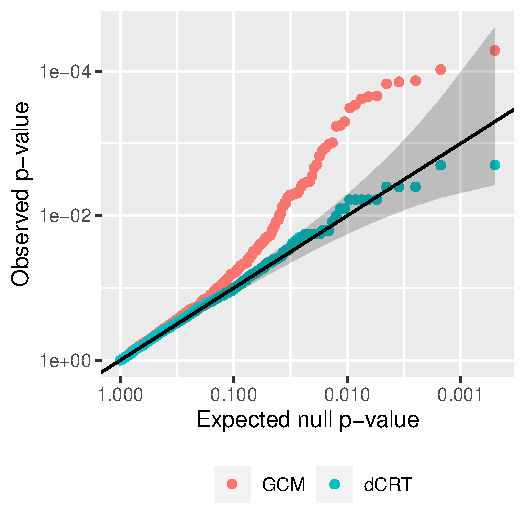
\includegraphics[width=\linewidth]{Figures/Q1/qq-plots.pdf} \\
    \end{subfigure}%
    \begin{subfigure}{0.5\textwidth}
        \centering
        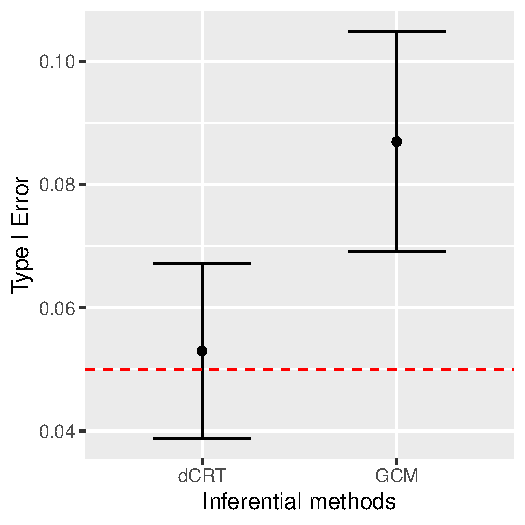
\includegraphics[width=\linewidth]{Figures/Q1/type_I_err_5e-2.pdf} \\ 
    \end{subfigure}

    \begin{subfigure}{0.5\textwidth}
        \centering
        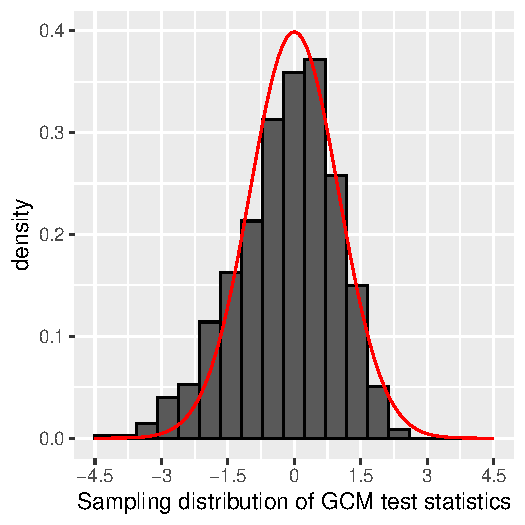
\includegraphics[width=\linewidth]{Figures/Q1/sampled-test-stats.pdf} \\ 
    \end{subfigure}%
    \begin{subfigure}{0.5\textwidth}
        \centering
        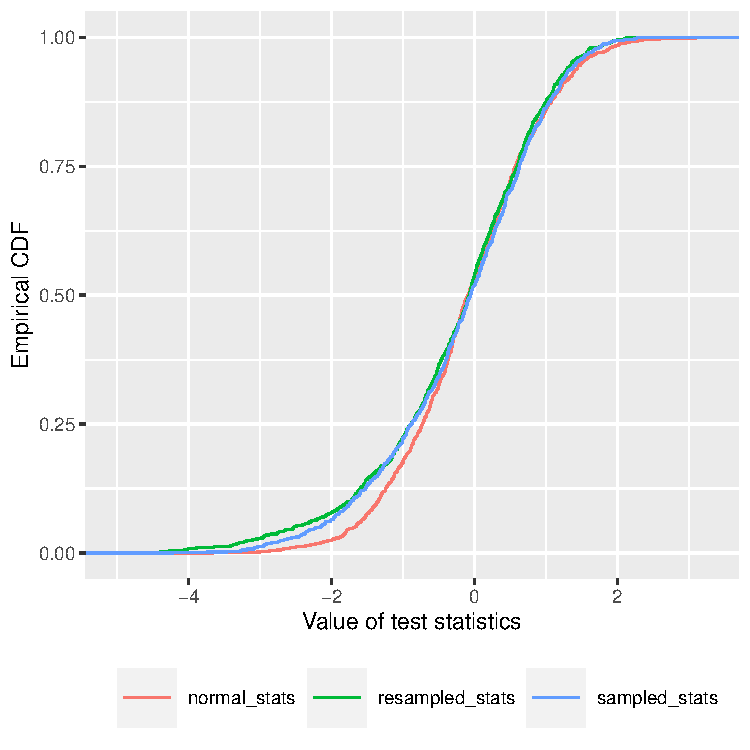
\includegraphics[width=\linewidth]{Figures/Q1/ecdf_comparison.pdf}
    \end{subfigure}
    \caption{Type-I error and MSE comparison when $\bm Y|\bm Z$ is a $\mathrm{Poisson}$ model.}
    \label{fig:dCRT_GCM_binomial_poisson} 
\end{figure*}



\section{Simulation study for the second (and partly the third) question}

To answer this question, we investigate into the following conditional models 
\begin{align*}
    \text{Poisson}(\exp[(-4,\bm Z^\top) \beta]),\ \text{Bern}(\text{expit}[(-3, \bm Z^\top)\beta]),\ N((0,\bm Z^\top)\beta,1)
\end{align*}
where $ \beta=\bm 1_{d+1}=(1,\ldots,1)^\top\in\mathbb{R}^{d+1}$. It is well-acknowledged that the Poisson regression is more 
difficult to fit than the logistic regression and the Gaussian regression. This motivates us to vary the choice of $\bm X|\bm Z$ 
while fixing $\bm Y|\bm Z\sim \text{Poisson}(\bm Z^\top\beta)$. Consider 
\begin{enumerate}
    \item[(1)]$\bm X|\bm Z\sim N(\bm Z^\top\beta,1),\bm Y|\bm Z\sim \text{Poisson}(\bm Z^\top\beta)$;
    \item[(2)]$\bm X|\bm Z\sim \text{Bern}(\bm Z^\top\beta),\bm Y|\bm Z\sim \text{Poisson}(\bm Z^\top\beta)$.
\end{enumerate}
To study how the strategy of resampling affect Type-I error, we include both the resampling from $\hat{\mathcal{L}}(\bm X|\bm Z)$ and 
from $\hat{\mathcal{L}}(\bm Y|\bm Z)$ and denoted the procedures as $\mathrm{dCRT}\_\text{X}$ and $\mathrm{dCRT}\_\text{Y}$ respectively. 
For comparison, we also incorporate the results of $\mathrm{GCM}$. The parameter setting is $n=100$ and $d$ is varied within $11$ to $15$ 
with space $1$. The simulation is repeated $10000$ times and the results are summarised in Figure \ref{fig:dCRT_GCM_asymmetry}. 

Clearly, we can see the discrepancy of the Type-I error between $\mathrm{dCRT}\_X$ and $\mathrm{dCRT}\_Y$. Since it is a only a conjecture 
that $\mathrm{Poisson}$ model is hard to fit, we further verify it by comparing the mean squared error (MSE) of the estimated $\mu_{n,x}(\cdot)$ 
and $\mu_{n,y}(\cdot)$. The results are shown in the bottom row of Figure \ref{fig:dCRT_GCM_asymmetry}. The much larger MSE of $\mu_{n,y}(\cdot)$
indicates that the $\mathrm{Poisson}$ model is indeed harder to fit. 


\begin{figure}[ht]
    \begin{subfigure}{0.5\textwidth}
        \centering
        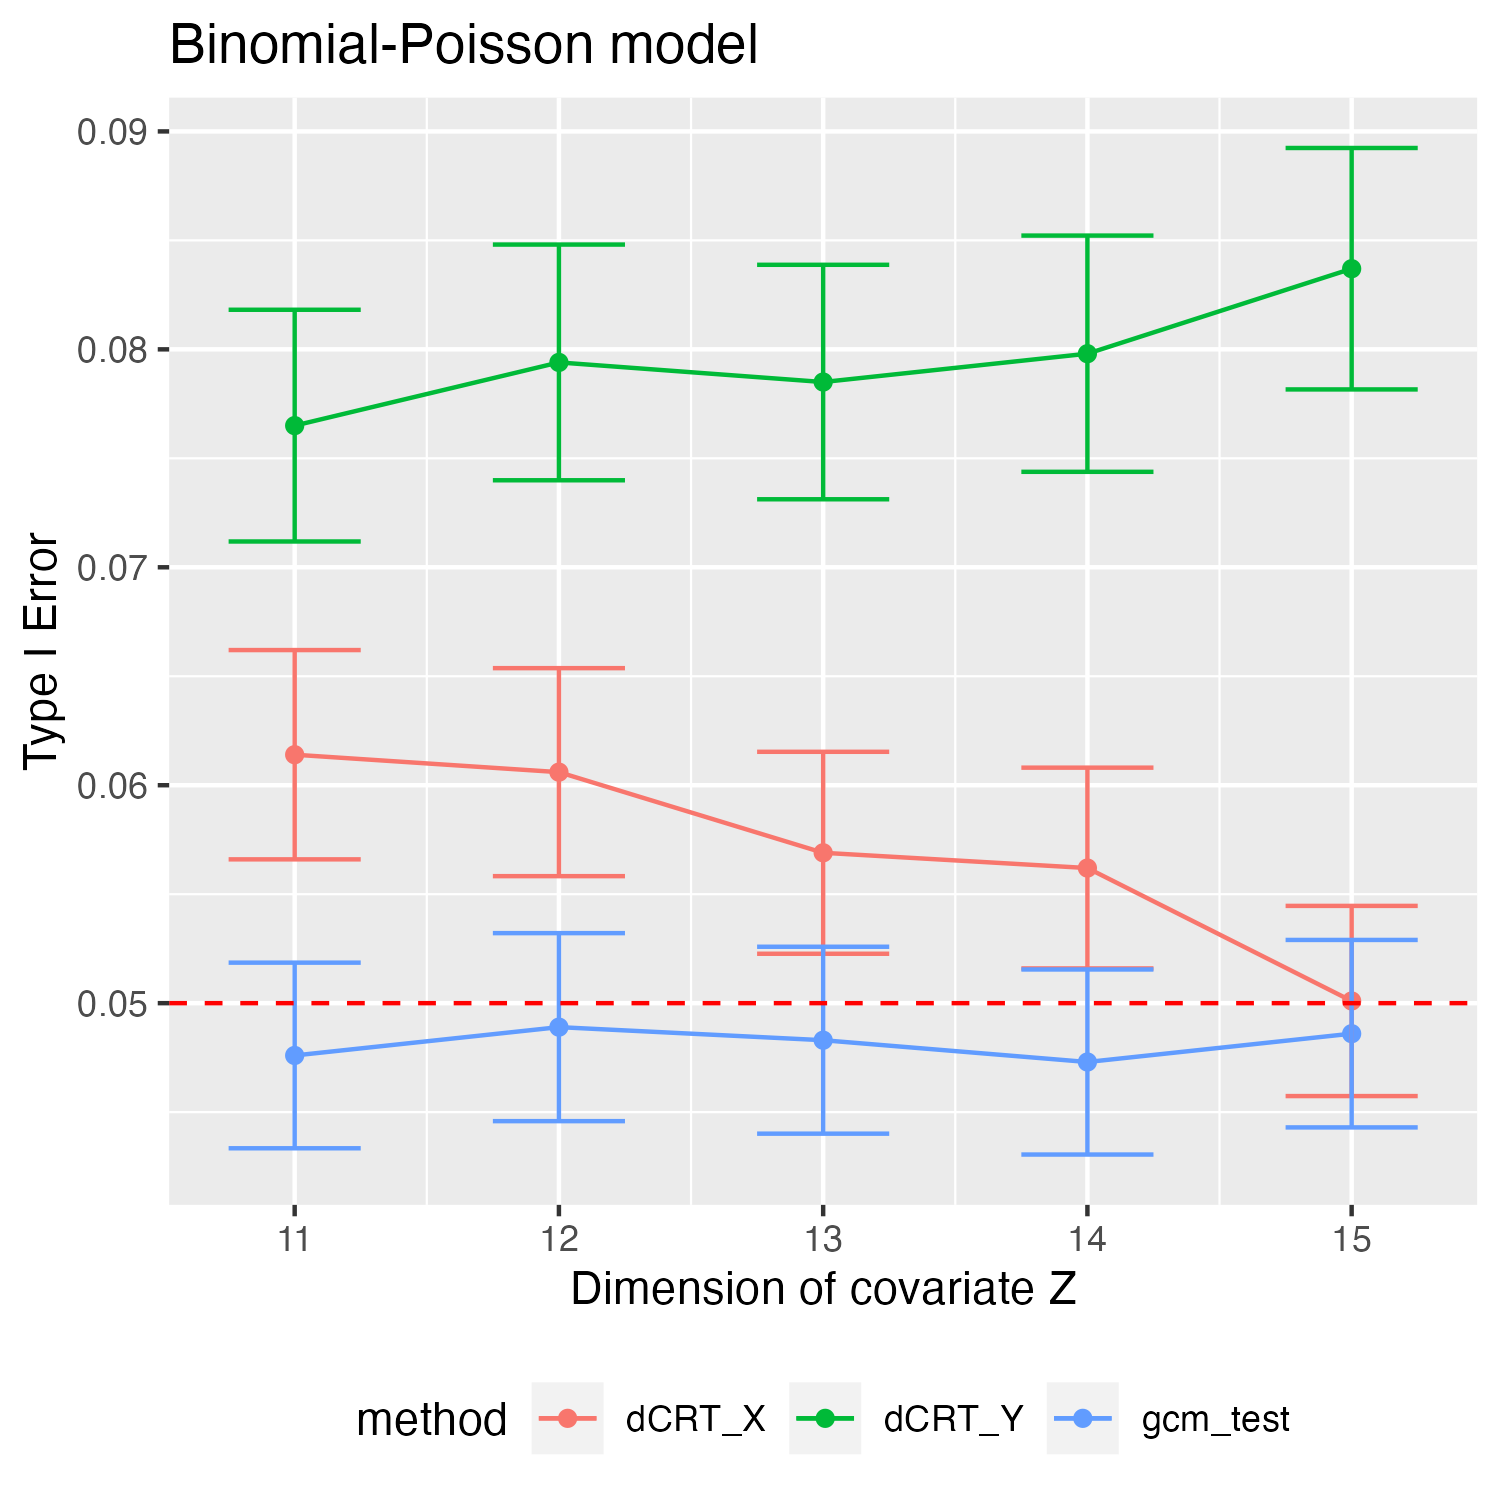
\includegraphics[width=\linewidth]{Figures/Q2/varying-dimension-binomial-poisson.png}
    \end{subfigure}%
    \begin{subfigure}{0.5\textwidth}
        \centering
        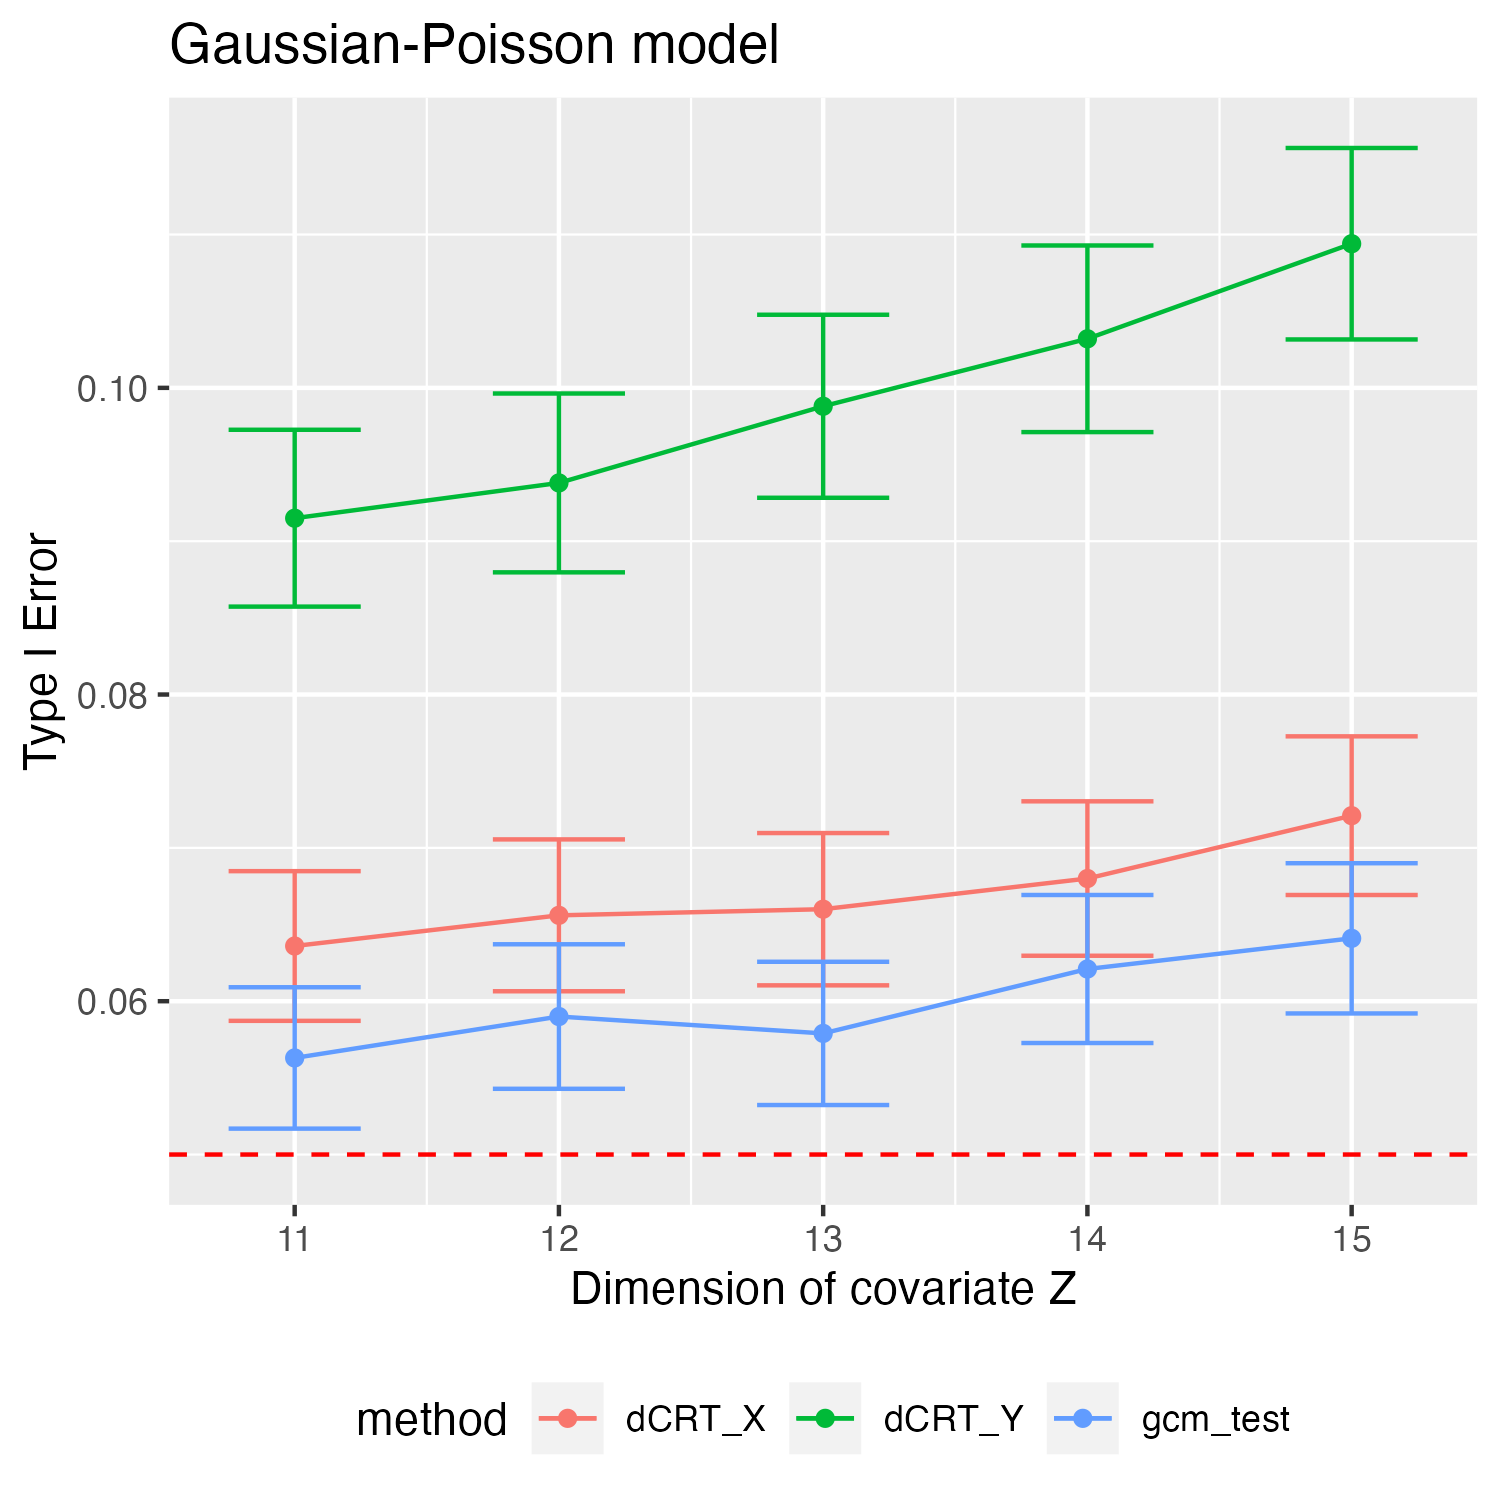
\includegraphics[width=\linewidth]{Figures/Q2/varying-dimension-gaussian-poisson.png} 
    \end{subfigure}

    \begin{subfigure}{0.5\textwidth}
        \centering
        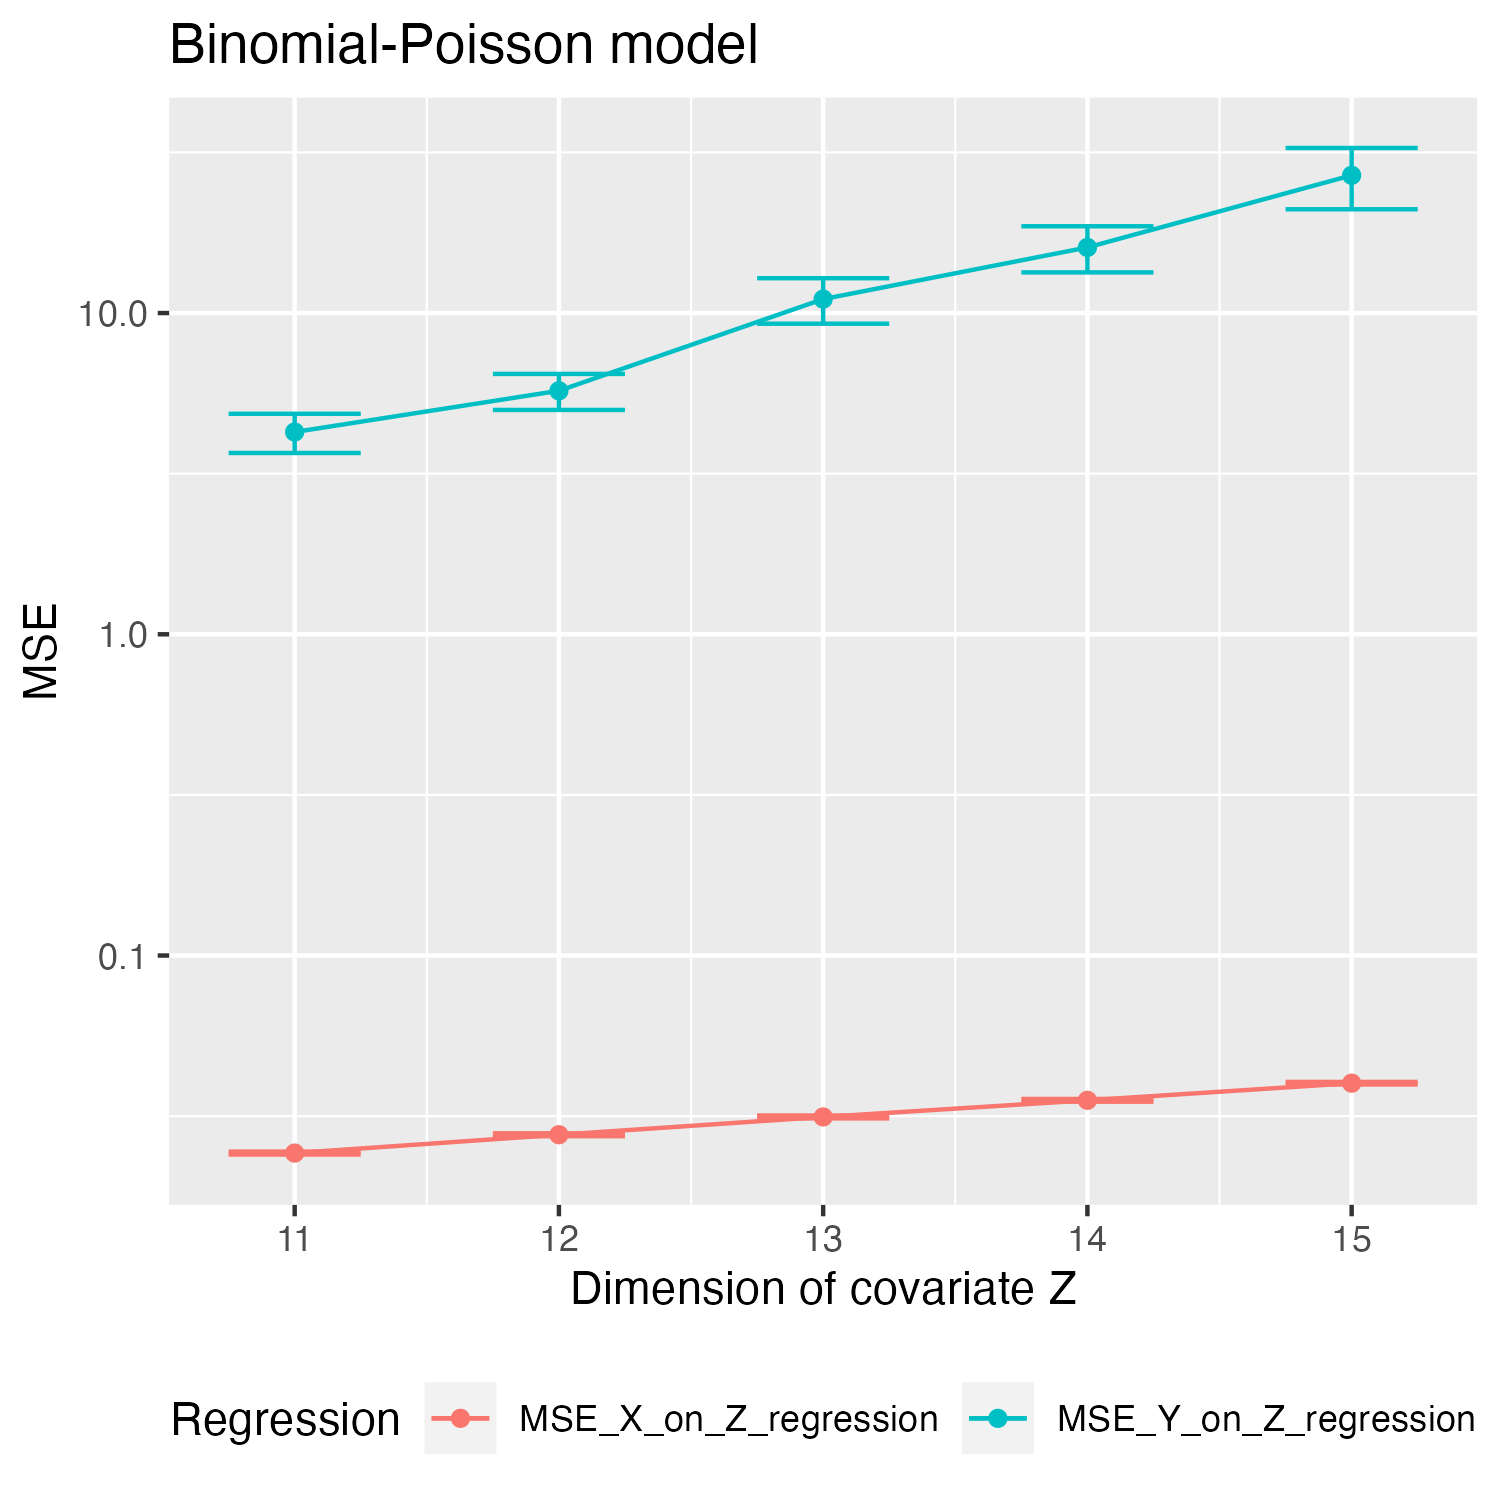
\includegraphics[width=\linewidth]{Figures/Q2/MSE-binomial-poisson.png}
    \end{subfigure}%
    \begin{subfigure}{0.5\textwidth}
        \centering
        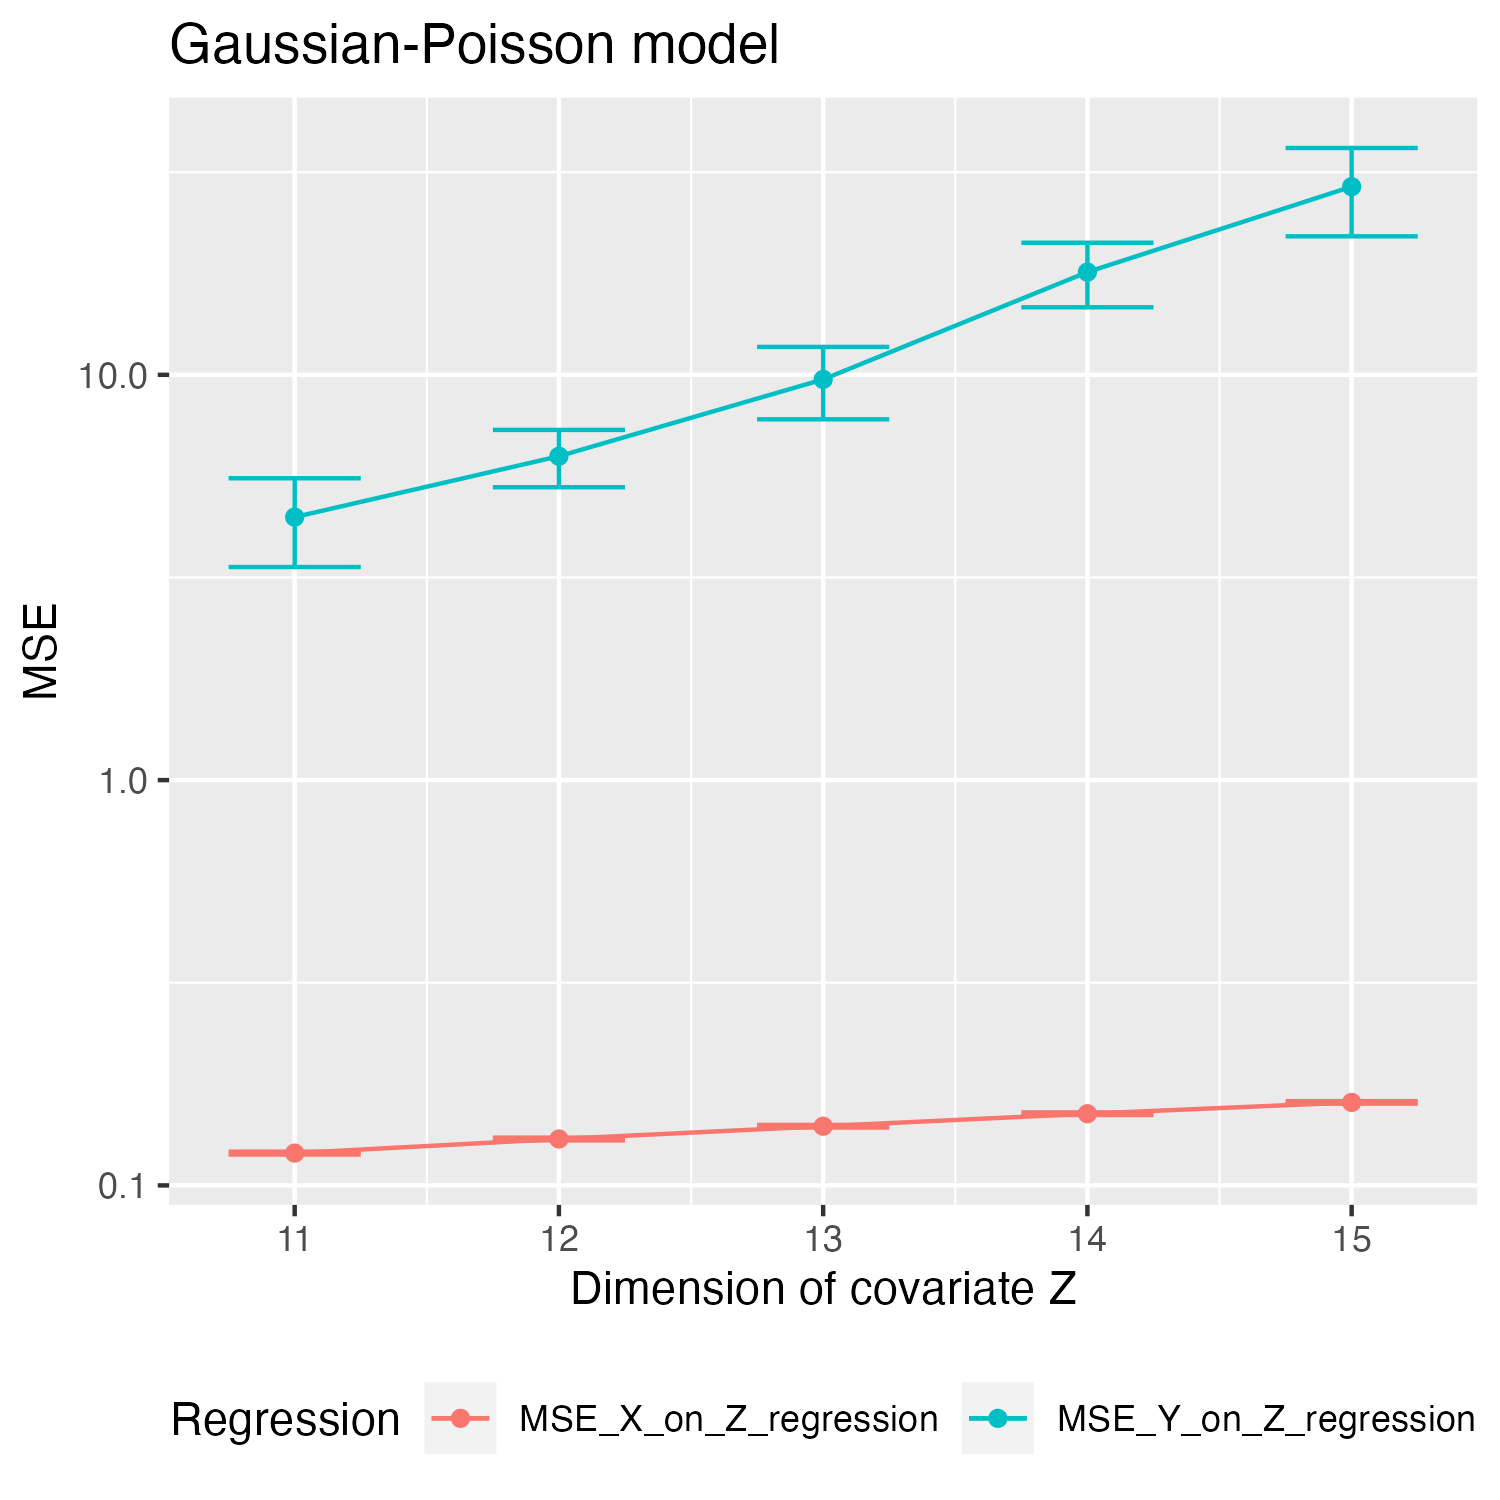
\includegraphics[width=\linewidth]{Figures/Q2/MSE-gaussian-poisson.png}
    \end{subfigure}
    \caption{Type-I error and MSE comparison when $\bm Y|\bm Z$ is a $\mathrm{Poisson}$ model.}
    \label{fig:dCRT_GCM_asymmetry} 
\end{figure}


\newpage
{\scriptsize
\printbibliography
}

\newpage



%%%%%%%%%%%%%%%%%%%%%%%%%%%%%%%%%%%%%%%%%%%%%%%%%%%%%%%%%%%%%%%%%%%%%%%%%%%%%%%%%%%%%%%%%%%%%%%%%








\end{document}

